% To be submitted for Text2KG Workshop 2023 colocated with EWSC 2023
% https://aiisc.ai/text2kg2023
% Series: https://scholia.toolforge.org/event-series/Q116982161
% Deadline 2023-03-15
% max 16 pages for full paper - 7 for short paper
% Previous Proceedings at https://ceur-ws.org/Vol-3184/
% 
% Graphics:
% https://docs.google.com/presentation/d/1a0YkKEDh_dcluTwEKJXxfpPKYPLGFQxBi2Lh_apR2UA/edit?usp=sharing
\documentclass[]{ceurart}
\usepackage[utf8]{inputenc}
\usepackage{wrapfig}
% render SVG files: https://tex.stackexchange.com/questions/122871/include-svg-images-with-the-svg-package
\usepackage{svg}
\usepackage{graphicx} % Required for inserting images
% define some macros/commands
% for tables
\usepackage{tabularx}
% source code rendering
\usepackage{minted}
\newcommand{\orcidID}[1]{\href{https://orcid.org/#1}{
\includegraphics[width=8pt]{orcid.png}}}
% typographical quoting
\newcommand{\tquote}[1]{``#1''}
% footnotelink
\newcommand{\footnotelink}[2]{\href{#1}{#2}\footnote{#1}}
% define some macros/commands
\newcommand{\wdq}[2]{\footnotelink{https://www.wikidata.org/wiki/#2}{#1 (#2)}}
\newcommand{\wdp}[2]{\footnotelink{https://www.wikidata.org/wiki/Property:#2}{#1 (#2)}}

\newcommand{\wdpTable}[2]{\href{https://www.wikidata.org/wiki/Property:#2}{#1 (#2)}}
\newcommand{\wdqTable}[2]{\href{https://www.wikidata.org/wiki/#2}{#1 (#2)}}
%double blind handling
% hiding with soul package - text still available in pdf
% couldn't get this to work
%\usepackage{xcolor}
%\usepackage{soul}
%\sethlcolor{yellow}
%\newcommand{\hide}[1]{\hl{#1}}
% censor package
% does not work properly
%\usepackage{censor}
%\newcommand{\hide}[1]{\censor{#1}}
% https://tex.stackexchange.com/a/95122/200531
% see also %https://www.alanshawn.com/latex3-tutorial/#macro-expansion-control-v
\usepackage{xparse,expl3}
\ExplSyntaxOn
\NewDocumentCommand{\regexreplace}{mmm}
{
  % set the token list to the third parameter 
  \tl_set:Nn \l_tmpa_tl {#3}
  % apply the regular expression #1 replacing with #2
  \regex_replace_all:nnN {#1} {#2} \l_tmpa_tl
  %\tl_replace_all:Nnn \l_tmpa_tl {#1} {#2}
  % use the resulting token list 
  \tl_use:N \l_tmpa_tl
}
\ExplSyntaxOff
\newif\ifreview\reviewfalse
\ifreview
\newcommand{\hide}[1]{\regexreplace{ [a-zA-Z] }{ x } {#1}}
%{■■■■■■■■■■■■■■■■■■■■■■■■■■■■■■■■■■■■■■■■■■■■■■■■■■■■}} 
\newcommand\simplehide[1]{#1}
\newcommand{\hiddenfootnotelink}[3]{\footnotelink{#2}{#3}}
\else
% cancel hiding
\newcommand{\simplehide}[1]{#1}
\newcommand{\hide}[1]{#1}
\newcommand{\hiddenfootnotelink}[3]{\footnotelink{#1}{#3}}
\fi

\begin{document}
\title{Semantification of CEUR-WS with Wikidata as a target Knowledge Graph}
\copyrightyear{2023}
\copyrightclause{Copyright for this paper by its authors.
  Use permitted under Creative Commons License Attribution 4.0 International (CC BY 4.0).}
\conference{Text2KG 2023: Second International Workshop on Knowledge Graph Generation from Text, May 28 - Jun 1, 2023, co-located with Extended Semantic Web Conference (ESWC), Hersonissos, Greece}
\author[1]{\simplehide{Wolfgang Fahl}}[
    orcid=0000-0002-0821-6995,
    email=fahl@dbis.rwth-aachen.de
]
\author[1]{\simplehide{Tim Holzheim}}[
    orcid=0000-0003-2533-6363,
    email=tim.holzheim@rwth-aachen.de
]
\author[1,2]{\simplehide{Christoph Lange}}[
    orcid=0000-0001-9879-3827,
    email=lange@cs.rwth-aachen.de
]
\author[1,2]{\simplehide{Stefan Decker}}[
    orcid=0000-0001-6324-7164,
    email=decker@dbis.rwth-aachen.de
]
\address[1]{\simplehide{RWTH Aachen University, Computer Science i5, Aachen, Germany}}
\address[2]{\simplehide{Fraunhofer FIT, Sankt Augustin, Germany}}

\date{March 2023}
%\begin{document}

%% Rights management information.
%% CC-BY is default license.
\begin{abstract}
For modern scholarly communication infrastructure, knowledge graphs are already ubiquitous. Some platforms of the publication lifecycle still struggle with catching up. In this paper, we use the example of the CEUR-WS publishing platform to show a viable approach to transition from a traditional HTML/PDF/text based environment to a single point of truth that separates the data and metadata storage from its presentation. This is possible using a public infrastructure such as Wikidata, which minimizes the maintenance effort and improves the publishing workflow.

The CEUR Workshop Proceedings (CEUR-WS) publishing platform (https://ceur-ws.org/) has been introduced in 1995 as a means to publish proceedings of scientific workshops (and smaller conferences) in computer science. 

Technically HTML, PDF and a filesystem directory hierarchy are the core formats being used and delivery is via the HTTP and FTP protocols. 

There have been multiple attempts in the past to make the metadata of the CEUR-WS platform available for computer based analysis and querying. None of these attempts has been consistent and continuous so far.

We report on the successful start of semantification of CEUR-WS with Wikidata as a target knowledge graph with the goal to achieve consistency and continuity for the future. 

The challenge was in handling the textual natural language description parts of the CEUR-WS content that is inherently still part of the semi-digitized approach of using HTML and PDF. We propose to have a better separation of concerns of metadata, display and storage and started implementing it.
\end{abstract}
\begin{keywords}
  Publishing\sep
  Information Extraction\sep
  Knowledge Graph\sep
  Linked Data\sep
  Metadata Extraction\sep
  Named Entity Linking\sep
  Named Entity Recognition\sep
  NLP \sep
  RDF \sep
  Semantification \sep
  Semantic Web\sep
  Wikidata
\end{keywords}

\maketitle

\section{Introduction}\label{sec:Introduction}
Modern scientific publishing infrastructure uses knowledge graphs as a native basis. \footnotelink{https://scholar.google.com/}{Google Scholar} is a popular and famous example. Microsoft Academic Graph~\cite{Wang2020} had the \tquote{graph} in its name. Although Microsoft terminated the service by end of 2021 the idea and content has been picked up and extended by OpenAlex~\cite{Priem2022}. Publishing and indexing platforms that are based on older technology such as MARC~\cite{Ganseman2015}, PICA~\cite{Costers1997} or XML struggle to catch up but gradually move to graph based approaches as  \footnotelink{https://blog.dblp.org/2022/03/02/dblp-in-rdf/}{DBLP did in March 2022} by offering SPARQL dumps that may be queried, e.g., using the \footnotelink{https://qlever.cs.uni-freiburg.de/dblp}{QLever dblp SPARQL endpoint}~\cite{Bast2017}.

\subsection{CEUR Workshop Proceedings}
CEUR-WS is a free online service that provides open access to  proceedings of workshops (and smaller conferences) in the field of computer science and information technology, hosted by by RWTH Aachen University's Chair for Information Systems and Databases. CEUR-WS is operated by the CEUR-WS Editors -- a team of unpaid volunteers -- working as a non-profit organization. Over 3,300 Volumes containing over 65,000 PDF documents in total have been published until March 2023.

CEUR-WS does not use a Content Management System for publishing but relies on pure HTML and PDF for rendering its \footnotelink{https://ceur-ws.org}{public website}. The metadata for these publications is only indirectly available by indexing services such as dblp~\cite{Ley2009} and {K10plus}\cite{k10plus2019}\footnote{\url{https://dblp.org/}, \url{https://opac.k10plus.de}}. Unfortunately both dblp and k10plus do not have a complete set of metadata records for all volumes as of March 2023 and in both cases there is a delay of some weeks/months before new volumes are picked up for indexing.

\subsection{The Trend towards FAIR Data and Open Science: Semantification}
% FAIR Data Introduction - why is this relevant? EOSC, NFDI, Open Access, Open Science
% FAIR Data as a basis for Knowledge Graphs
Since inception the FAIR principles~\cite{Wilkinson2016} have been a  success. They have been adopted by various industries (e.g., the pharmaceutical industry) and national and international projects (e.g., the Common European Dataspaces). 
Persistent Identifiers (PIDs) and rich metadata are the core components of the FAIR principles, and they provide the means to create Knowledge Graphs~\cite{Cousijn2021} .

Representing digital traces of scholarly communication in Knowledge Graphs (KGs)~\cite{Hogan_2021} is useful for supporting use cases such as literature search and recommendation of events for attendance or publishing. The metadata of the most relevant entities as outlined in Figure~\ref{fig:core_entities}\footnote{The original SVG graphic is clickable and leads to the corresponding Wikidata properties and entity types} need to be made available to offer such a knowledge graph.

\begin{figure}
    \centering
    \includesvg[width=\linewidth]{CoreEntities.svg}
    \caption{Most relevant entities for scientific publishing -- the entities at the core of this work are blue}
     \label{fig:core_entities}
\end{figure}

The term \tquote{Semantic Web}~\cite{BernersLee2001} has been coined by Tim-Berners Lee et al.\ to describe the effect of resources on the Web interlinked making use of such metadata.
Therefore we choose \tquote{Semantification} as the title of the project and this paper to describe the process of creating a Knowledge Graph and making the results available in Semantic Web fashion. The Semantification of CEUR-WS has been attempted multiple times in the past~\cite{Lange2014,Sateli2015} -- always under the assumption that a local RDF/SPARQL endpoint would be the goal to achieve. The results have not been consistent and durable since the publishing workflow has not been adapted and the single point of truth for the metadata is still buried in the HTML/PDF/text documents. The fear of maintenance follow-up problems, given that CEUR-WS is a non-profit service with no budget, was a major obstacle. 

\subsection{Challenges in making CEUR-WS more FAIR via Semantification}\label{sec:fair_challenges}

To semantify CEUR-WS, the following requirements where most relevant:
\begin{itemize}
    \item the metadata should follow the FAIR \cite{GOFAIR2019,Wilkinson2016} principles 
    \begin{itemize}
    \item F1: (Meta)data are assigned globally unique and persistent identifiers (see Section~\ref{sec:event_pids}).
     \item F2: Data are described with rich metadata.
      \item F3: Metadata clearly and explicitly include the identifier of the data they describe.
      \item F4: (Meta)data are registered or indexed in a searchable resource.
    \end{itemize}
    \item relevant queries should be supported, as derived from the original set of queries of the 2014 Semantic publishing challenge as outlined in Section~\ref{sec:sempub_challenge}
    \item the metadata should reuse an established ontology
    \item the manual and automatic curation of entries should be possible with public access for all stakeholders, e.g., editors, authors, organizers, publishers, indexers
    \item the infrastructure should be stable and there should be sufficient trust in its long term availability
    \item an open source non-profit infrastructure is preferred since this is also the mode of operation of CEUR-WS
\end{itemize}

Given the HTML/PDF/text input of CEUR-WS, we need to create the corresponding Knowledge Graph and separate the single-point-of-truth computer readable metadata from the different representations such as HTML so that the above requirements are fulfilled. 

%The \footnotelink{https://cr.bitplan.com/index.php/Semantic\_Publishing\_Challenge}{original task} called for 20 such queries to be answerable. 
%Formally we need to implement a function hat takes two Trees (IT,PT) as an Input and outputs a Graph G=(V,E).

%The IT Tree is the HTML Dom Tree of the CEUR-WS index page where the leaves are HTML markup nodes that might be annotated with an attempted RDFa syntax. 

%The PT Tree is a three level filesystem /HTML Dom tree of 
%Directories per volumes - with an index HTML DOM Tree for the volume and a list of individual PDF files per paper of the volume.

%The leaf node contents are the PDF contents of the files and the HTML markup nodes of the Volume index page.
Both the HTML and PDF encoding of the original scientific content are structured for the purpose of optimizing the display / output on paper or screens; therefore, there is a structure loss compared to what was originally available in the text document processor files that the authors might have been using~\cite{Fahl2023}. In Figure~\ref{fig:digital_publishing} shows the part of the publishing process where the rendering step causes this loss. Most scholars are not aware of this loss in the daily use of published content just because the documents are optimized for display and human consumption~\cite{Yu2020}. For the metadata extraction and use in knowledge graphs the difference is sometimes disastrous, e.g., when a simple text from a PDF document can not be extracted any more due to exotic styling and formatting or simply because only a scanned graphic image version of an older document is available that needs Optical Character Recognition to extract the textual content.  

\begin{figure}
    \centering
    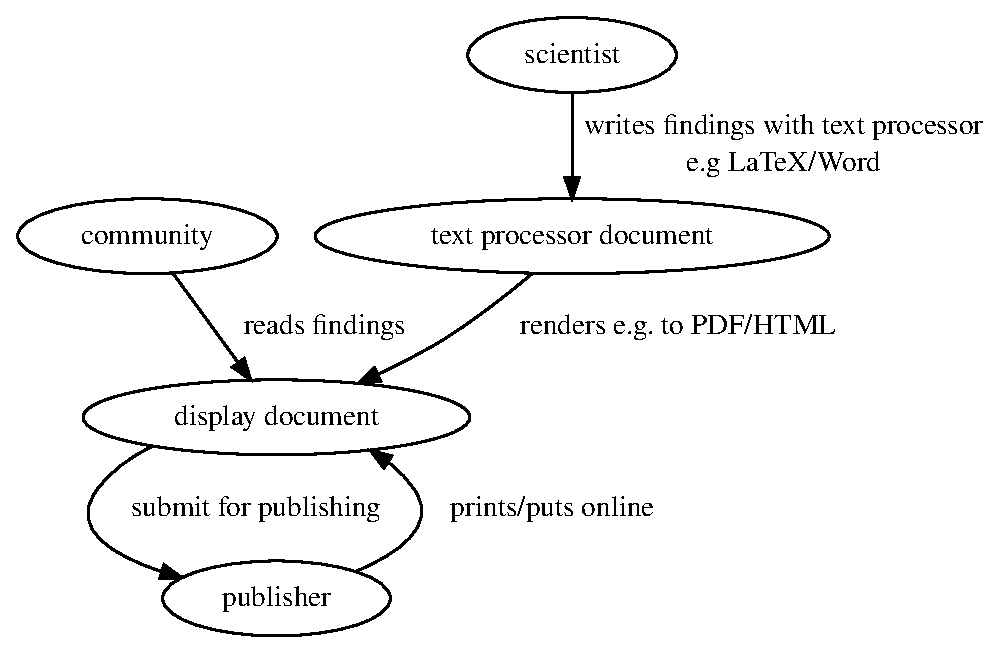
\includegraphics[width=0.7\linewidth]{DigitalScientificPublishing.eps}
    \caption{Textprocessing step of digital Scientific Publishing}
     \label{fig:digital_publishing}
\end{figure}

The metadata needed for creating the knowledge graph is only available in natural language/text form and follows rules that have been changed multiple times during the history of CEUR-WS. From 2013 to 2023, there have been 33 different versions of the index file template with no proper tracing of what was changed from version to version. 

% https://cr.bitplan.com/index.php/CEUR-WS_Versions
\subsection{Contributions of this Paper}
Our first contribution is to provide the tools, infrastructure and approaches to modify the CEUR-WS publication workflow to consistently supply FAIR high quality metadata (Semantification). 

Secondly, splitting the metadata for the three main entities Event, Event Series and Proceedings is a major step towards improving the metadata quality, e.g., by allowing event series data to be checked for completeness and be completed from different sources where possible. Unfortunately, currently non of the stakeholders have the motivation to do this completion, while it is valuable, e.g., for assessing the quality of an event series. The necessary change of perspective to convince the stakeholders is a chicken-egg problem, which the CEUR-WS semantification will help to facilitate. 

Provide a bootstrapping~\cite{Bardini2001,Engelbart2007} approach to allow for getting rid of manual editing of the CEUR-WS website content and instead using a CMS approach based on the single-point-of-truth metadata that separates the concerns of storage and display. Making sure the results are already visible and usable during the ongoing project.

These contributions are fit to be generally applied to other publishing use cases.

\section{Related Work}\label{sec:Related Work}
%BrylEtAl
\subsection{Semantic Publishing challenge}\label{sec:sempub_challenge}
The Semantification of CEUR-WS has been publicly pursued by the Semantic Publishing challenge~\cite{Lange2014} from 2014. Given an excerpt of CEUR-WS, scholars were asked to prepare a RDF knowledge graph to allow for a set of 20 queries to be answered to complete Task~1.

% https://ceur-ws.bitplan.com/index.php/Vol-3184/paper7
% https://github.com/angelobo/SemPubEvaluator
One \footnotelink{https://github.com/ceurws/lod/wiki/SemPub2015}{original task of the Semantic Publishing Challenge (SemPub2015)} read as follows:
\textit{Task 1: Extraction and assessment of workshop proceedings information.
Participants are required to extract information from a set of HTML tables of contents, partly including microformat and RDFa annotations but not necessarily being valid HTML, of selected computer science workshop proceedings published with the CEUR-WS.org open access service. The extracted information is expected to answer queries about the quality of these workshops, \dots}. 

Kolchin et al.~\cite{Kolchin2014,Kolchin2015} have submitted results to the challenge twice with an approach using XPath Queries on the HTML DOM markup and converted the results directly to triples; see \footnotelink{https://github.com/ailabitmo/ceur-ws-lod}{ceur-ws-lod repository on GitHub}. 
The reusability of this approach is limited since the parsing and generation code are intermixed.

Sateli and Witte~\cite{Sateli2015} applied the GATE framework~\cite{Cunningham_2001, Cunningham_2013} and a pipeline to create triples from the parsing result~\cite{Sateli2016}; see also \footnotelink{https://www.semanticsoftware.info/sempub-challenge-2015}{their supplementary material}. 

The 2015 work of Milicka and Burget~\cite{Milicka2015} used \footnotelink{https://github.com/FitLayout/ToolsEswc/tree/master/awk}{awk text pattern matching} as a tool to parse the table of content files per Volume.

The objective of these attempts was to create a local SPARQL endpoint to allow to perform the required queries and fulfill the role of a target knowledge graph and point of truth. 

Tasks 2 and 3 called for the detailed analysis of the PDF files.

All challenge contributions had a purely scientific focus and where not fit for making the results operational and being used in the actual CEUR-WS publishing workflow. 
\subsection{Persistent Identifiers in a scholarly publishing context}\label{sec:event_pids}
A study about Linked Data~\cite{Kafer2013} found that each year about 10\% of Linked Data URIs are no longer dereferencable.
One way to mitigate the issue is to introduce persistent identifiers (PIDs), which aim to fulfill the following principles~\cite{Sollins2012}: longevity, scalability, extensibility, and security.
As noted in~\cite{kunze-ark-36}, the importance to ensure the longevity of PIDs is that \tquote{persistence is purely a matter of service}.
Thus, PIDs can only remain persistent if someone is committed to ensuring they stay accessible to users.
This requires an engagement or a service level agreement for PID availability, in contrast to URIs, where no such agreement exists.

As \cite{Cousijn2021} notes, PIDs can be resolved via a URI, which follows the first principle of the Den Haag Manifesto from 2011\footnote{\url{https://doi.org/10.5281/zenodo.55666}}.
With this alignment, Semantic Web tools, standards, and concepts to link, map, query, and integrate different data formats and data sources, and knowledge graphs become usable data based on the FAIR data principles. 

Franken et al.~\cite{Franken2022} have promoted the idea of using persistent identifiers (PIDs) for scientific events in the same way as there are already persistent identifiers for papers (DOI), people (ORCID), organisation (GRID, ROR) and books (ISBN).  They argue that it is also becoming more and more common practice to use PIDs to identify other important entities or objects.
But as mentioned by Bryl et al.~\cite{BrylEtAl:SePublica2014}, it will only be beneficial if more metadata is provided and the PID is actively used to interlink with other entities.
%The use of DOIs for this purpose is recommended because of the broad adoption of DOIs and the possibility to link to the ConfIDent platform and use it as a marketing tool for that project. 

Introducing PIDs in form of DOIs to CEUR-WS brings up the follow-up problem of who should be responsible for minting the DOIs, when the minting should be done and what the target URL of the DOI should be - not all organizers might like the landing page not to be under their own control. Wikidata Entity identifiers (Q-identifiers) seem to be a better alternative, since a rich set of other identifiers may be linked to any Wikidata Entity including DOIs, homepages and local and internationally known library and commercial and non-commercial indexing service identifiers.

\subsection{Metadata Extraction from PDF, HTML and Text} 

As part of the \footnotelink{https://github.com/WDscholia/scholia/issues/1438}{Scholia Open Source Project}, Nielsen~\cite{Nielsen2017} created a scraper tool capable of creating QuickStatements~\cite{Manske2016} output; see \footnotelink{https://github.com/WDscholia/scholia/blob/master/scholia/scrape/ceurws.py}{scrape/ceurws.py}. Using the scrape/QuickStatements chain allows for creating Wikidata entries for each paper. The \footnotelink{https://www.wikidata.org/wiki/Q117040467}{Vol-3184/paper4} Wikidata entry has been created this way by us to show the effect. Unfortunately, the \wdp{author name string}{P2093} property is used instead of immediately doing the disambiguate step for the author strings. 

\footnotelink{http://ptp.bitplan.com}{Proceedings Title Parser}~\cite{Fahl2022} 
has a CEUR-WS parsing mode, which already had the RDFa extractor capability (allowing to cover more recent CEUR-WS volumes using that markup style). Part of this work has been reused and extended to a fully fledged parser in the work we are reporting here.

CERMINE (Content ExtRactor and MINEr)~\cite{Tkaczyk_2015} is a software library and a  \footnotelink{http://cermine.ceon.pl}{web service} for extracting metadata and content from PDF files containing academic publications.
The text content is analysed and a structured XML document containing metadata on, e.g., authors and citations created~\footnote{See CEUR-WS Volume 3352/Paper1.pdf example \url{https://cr.bitplan.com/index.php/CERMINE/Example}}.
The lookup features of CERMINE are limited, e.g., to finding the ISO country code of the country of an institution an author is affiliated with.

GROBID (GeneRation Of BIbliographic Data)~\cite{Lopez_2009} has been gradually extended to be a machine learning library for extracting, parsing and re-structuring raw documents such as PDF into structured XML/TEI encoded documents with a particular focus on technical and scientific publications. We have tried out GROBID on over 50,000 papers so that the results are now a further potential source for disambiguation according to the original tasks 2 and 3.

\section{CEUR-WS Semantification}\label{sec:Semantification}

\subsection{Overview}\label{sec:sem_overview}
Figure~\ref{fig:ceurmake_workflow} shows the overview of the CEUR-WS Semantification workflow.
The workflow is cyclic -- it starts with what has so far been the single point of truth metadata, i.e., the ones embedded in the HTML/PDF/text of the static publication infrastructure. The Metadata Extraction step parses the input files and creates Metadata Records (which are cached as JSON records and in an SQLite relational database). These form the basis for the Matching/Reconciliation that queries Wikidata, dblp and GND with the respective SPARQL endpoints. The semantified Metadata Records are now available and may be stored in the format we see fit with JSON being the intended format for the upcoming project phase. In the next cycle the parsing of existing records is not necessary any more as long as there have been no changes. When new volumes are published, the main page, listing all proceedings volumes, is modified and HTML tables of content and PDF files are added per volume as submitted by the workshop editors.  

%\subsection{Steps}
%* Person disambiguation
%** Editor disambiguated with affiliation and homepage
%** id lookup orcid url is given as homepage
%* label lookup + majority vote
%** city and country are resolved to their Qid
%* date range (as text) is parsed from string to proper start and end date
%* NLP
%** ordinal is extracted from proceedings title
%** series title is extracted from proceedings title
%** event is extracted from proceedings title
%** event type (Conference or Workshop)
%* parsing of semi-structured data (html + css classes)
%** acronym
%** event website
%** publication date
%** paper and its authors
%*** Author disambiguation pending
%*** dblp lookup based on paper title → dblp author id

\begin{figure}
    \centering
    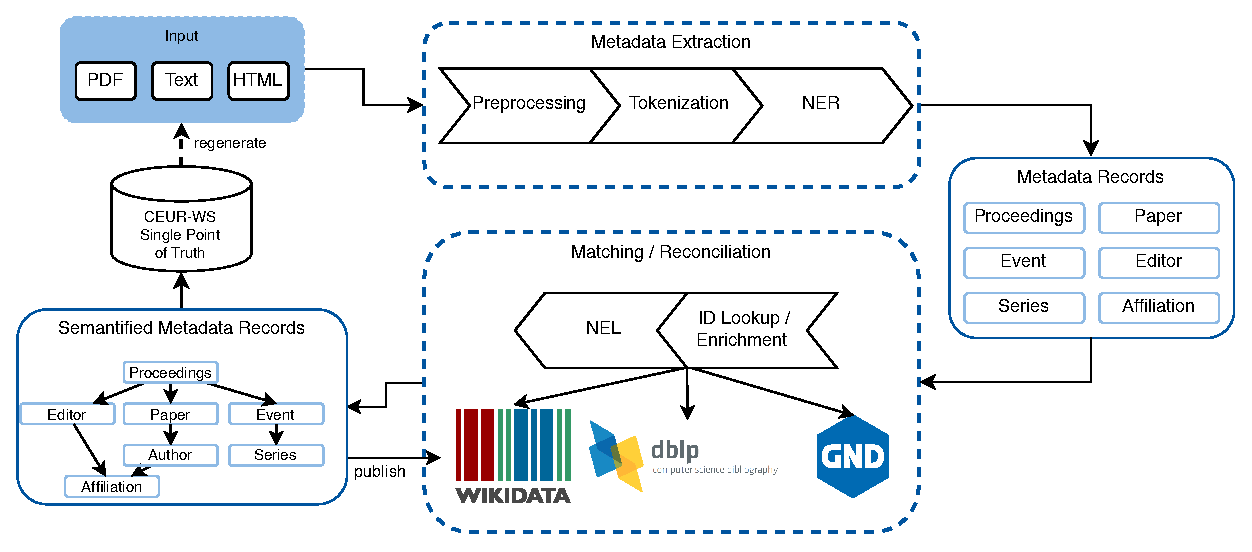
\includegraphics[width=\linewidth]{pyceurmake_workflow.eps}
    \caption{Workflow of the CEUR-WS Semantification}
    \label{fig:ceurmake_workflow}
\end{figure}

The steps of semantification workflow for CEUR-WS as depicted in Figure~\ref{fig:ceurmake_workflow} will be explained in the following.

\subsection{Preprocessing}
To extract the relevant markup elements we use the BeautifulSoup4 python library with additions to handle the RDFa-like annotations that have been applied in newer CEUR-WS volumes.
The main obstacle for the extraction of the markup elements is that so far 33 different versions have been used for the volume pages, which were often also edited manually, resulting in small differences even within the versions.
The usage of the different page versions follows a long-tail Zipfian distribution with 5 versions covering 60\% of all volumes.

\subsection{Tokenization}

\subsubsection{Disambiguation using Event Signatures}\label{sec:Event_signature}
As outlined in Section~\ref{sec:event_pids} PIDs would be useful for uniquely identifying scientific events. While PIDs are not available, it is necessary to use a quasi-identifier~\cite{OECD2008} consisting of a set of metadata elements that we call \tquote{Event Signature}. There is neither a standardized definition of event signatures nor a recommendation for their use in references and proceedings titles. Retrieving the signature from the volume's textual description is a core step in creating the CEUR-WS knowledge graph. 

\ifreview
In~\cite{Franken2022}, it has been shown
\else
As part of~\cite{Franken2022}, the main author has shown
\fi
that a typical scientific event \tquote{signature} consists of the following metadata (the example event being \footnotelink{https://www.wikidata.org/wiki/Q48027931}{ISWC 2019} \emph{The Semantic Web – ISWC 2019: 18th International Semantic Web Conference, Auckland, New Zealand, October 26–30, 2019}):
\begin{description}
\item[acronym] a short name for the conference, often consisting of 3 to 8 upper case letters trying to be unique but actually often being ambiguous.  For instance, ISWC may refer to the \textbf{International Semantic Web Conference} or to the International Symposium on Wearable Computing.
\item[frequency] annual, biennial, triennial -- most events have an \textbf{annual} frequency and this is mostly \textbf{not stated explicitly}.
\item[event reach] target reach of the conference such as \textbf{international}, European, East Asian
\item[event type] such as \textbf{Conference}, Workshop, Symposium  
\item[year] a two or four digit reference to the year in which the event took place -- not to be confused with the year of publication of the proceedings, which might be different (\textbf{2019})
\item[ordinal] often used to enumerate the conference series instances (\textbf{18th})
\item[date] start date and end date or date range of the conference (\textbf{October 26--30})
\item[location] description of the location of the conference often consisting of country, region and city -- sometimes with details about the exact venue. (\textbf{Auckland, New Zealand})
\item[title] the title often contains scope, type and subject of the conference (\textbf{International Semantic Web Conference})
\item[subject] description what the conference is about often  prefixed with ``on'' (\textbf{Semantic Web})
\item[delimiters] a variety of syntactic delimiters such as blanks, comma, colon, brackets are used depending on the citation style.
\end{description}

The event signature needs to be extracted from the CEUR-WS main and volume tables of content and stored as triples for the target KG. 

The distinction between proceedings, event and event series needs to be made -- therefore the result needs to be split and disambiguated against existing entries in the target KG.

The mapping as outlined in Table~\ref{tab:wikidata_mapping} has been used to map to the \tquote{event} and \tquote{proceedings} entry in Wikidata.  The top rows of the table show the common properties of the proceedings and event item entries, followed by the special properties for event followed by the special properties for proceedings.

The series entry for the Text2KG example has been created and the new \tquote{colocated} property is  filled for this example. The \footnotelink{https://scholia.toolforge.org/event-series/Q116982161}{Text2KG Workshop series scholia overview} shows the connections.

As an example, we are using the Wikidata entry for the \footnotelink{https://www.wikidata.org/wiki/Q113512465}{Text2KG@ESWC-2022} workshop, whose proceedings have been published as \footnotelink{https://ceur-ws.org/Vol-3184/}{CEUR-WS Volume 3184} with the \href{https://www.wikidata.org/wiki/Q113512180}{Wikidata proceedings item} being shared by another workshop (a special but still frequent case).

\begin{table}
\caption{Mapping Event Signature Elements to Wikidata}
\label{tab:wikidata_mapping}
%\begin{minipage}{\textwidth}
\begin{tabular}{p{2.5cm}p{3.7cm}p{6cm}}
\toprule
property & PID & example\\
\midrule
acronym     & \wdpTable{short name}{P1813} & Text2KG 2022 \\
title       & \wdpTable{title}{P1476} & 1st International Workshop \newline on Knowledge Graph Generation From Text \\
\midrule
event type  & \wdpTable{instance of}{P13} & Workshop\\
date(start) & \wdpTable{start time}{P580} & May 30th, 2022 → 2022-05-30\\
date(end)   & \wdpTable{end time}{P582} & May 30th, 2022 → 2022-05-30\\
location    & \wdpTable{location}{P276} & Hersonissos → \wdqTable{Chersonesos Irakliou}{Q1018106}\\
country     & \wdpTable{country}{P17}  & Greece → \wdqTable{Greece}{Q41}\\
series      & \wdpTable{part of the series}{P179}  &  International Workshop on Knowledge Graph Generation From Text → \wdqTable{Workshop on Knowledge Graph Generation From Text}{Q116982161}\\
ordinal     & \wdpTable{series ordinal}{P1545} & 1st\\
colocated with & \wdpTable{colocated with}{P11633} & ESWC 2022 → \wdqTable{ESWC 2022}{Q110791806}\\
homepage & \wdpTable{official website}{P856}& \href{ https://aiisc.ai/text2kg/
}{ https://aiisc.ai/text2kg/
}\\
\midrule
URN & \wdpTable{URN-NBN}{P4109} & urn:nbn:de:0074-3184-1 \\
publication date & \wdpTable{publication date}{P577} & 2022-08-11 \\
dblp id & \wdpTable{DBLP publication ID}{P8978} &  conf/esws/2022text2kg \\
k10plus id &\wdpTable{K10plus PPN ID}{P6721} & 1818588285\\
\bottomrule
\end{tabular}
%\end{minipage}
\end{table}

\subsection{Named Entity Recognition and Linking (NER \& NEL)}
The Named Entity Recognition (NER) and Named Entity Linking (NEL) tasks for the CEUR-WS Semantification are based on the textual input from the HTML markup that needs parsing into tokens that represent entities and then matching the textual content of the tokens against Wikidata entries that might need disambiguation. 
The semi-structured HTML markup helps hereby to reduce the input complexity for the parsing of the different entity types and therefore increases the accuracy of the matching process~\cite{COCHINWALA20011}.
Items to disambiguate are derived from the event signature as outlined in section \ref{sec:Event_signature}: Volumes, Papers, Editors, Authors, Locations (Country/Region/City), Dates, Ordinals, Acronym, Homepage.

For the phase of the project we are reporting, the mass creation of Proceedings and Event entries was in the focus. The Paper, Editor and Author disambiguation and Event series completion has been prepared and example results are available to show that the elements are available and may be systematically created and queried.
%as we intend to do  mass-creation of wikidata items after the green light from our legal department which is due after the publication of this work. 
%data reconciliation~\cite{MoEl1996}~\cite{KiCR2023}
\subsubsection{Location NER and NEL}
The location of an event is described in the table of contents in \textit{span} elements usually classified as \textit{CEURLOCTIME}.
Their value contains semi-structured information about the event's location and date range, e.g., \tquote{Hersonissos, Greece, May 30th, 2022}.
Besides the varying formats of the location and date definition the location information can be fairly easy separated from the date.
This leaves a string that should contain information about the city and country.
There exist cases were also the region or venue is named, and since more and more conferences moved to virtual meetings since 2020, the location string could also contain indications for that.
Since location string can be identified on extraction Named Entity Recognition (NER) and Named Entity Linking (NEL) are done in one step to get Wikidata Qids of the mentioned locations.
For the NEL we used geograpy3, a Python library that has a database with the labels of countries, regions and cities in multiple languages linking to the corresponding Wikidata Qid.
The response of this label lookup is a list of possible locations of the aforementioned categories.
The list is sorted by the category order city, region, country were the cities are also ordered by population.
To this list we apply again a ranking since we know that in most cases the country is named within the string so we can verify that we select a city were its country was also detected.
For the given example the result would then be \tquote{Hersonissos, Greece} → \wdq{Chersonesos Irakliou}{Q1018106} (\wdq{Greece}{Q41})


\subsubsection{Editors and Authors}
The author and editor name disambiguation is one of the main challenges of libraries and indexers~\cite{Subramanian_2021}.
Due to the common occurrence of duplicate names, abbreviations of first names, typos and encoding errors disambiguation is an expensive and error prone task if high accuracy is aimed.

In CEUR-WS, the editor information is given in an HTML element containing the editor signature usually given name and family name with a reference to the affiliations as shown in Listing~\ref{listing:editor_span}.
\begin{listing}
\caption{CEUR-WS volume page HTML markup excerpt of editor definition}
\label{listing:editor_span}
\begin{minted}{html}
<b> TEXT2KG edited by </b>
</p><h3>
   <span class="CEURVOLEDITOR">Sanju Tiwari</span> ... 1
   <span class="CEURVOLEDITOR">Nandana Mihindukulasooriya</span> ... 2
   <span class="CEURVOLEDITOR">Francesco Osborne</span> ... 3 4
   <span class="CEURVOLEDITOR">Dimitris Kontokostas</span> ... 5
   <span class="CEURVOLEDITOR">Jennifer D’Souza</span> ... 6
   <span class="CEURVOLEDITOR">Mayank Kejriwal</span> ... 7
</h3>
\end{minted}

\end{listing}
For newer publications ORCIDs of Authors and Editors might be directly available from the PDF input.
For older volumes, only the plain name, affiliation and no identifier is provided that could simplify the disambiguation.
Fortunately, around 80\% of the volumes are indexed at dblp.
dblp provides high quality disambiguated data about the proceeding editors and paper authors also accomplished through manual curation~\cite{Kim_2018}.
Therefore, extracting the editors and resolving the name to an identifier by looking up the dblp id seems to be the best option.
The same strategy as used for the editors also applies to the authors but here the affiliation needs to be extracted from the paper PDF.

\subsection{ID Lookup/Enrichment}
\subsubsection{dblp and k10plus Volume matching and linking}
dblp and k10plus records may be trivially matched by the unique identifier volume number of a proceeding combined with the URN of the CEUR-WS proceedings series.

We are using the QLever dblp SPARQL endpoint mentioned in Section~\ref{sec:Introduction} to match CEUR-WS volumes against dblp entries by volume number.

For the k10plus matching we use the catmandu library which allows to query the PICA~\cite{Costers1997} based k10plus database for URN matches see the  \footnotelink{https://w.wiki/6Qm5}{PPN/Volume/WikidataItem matching SPARQL Query}. 

Based on the resolved IDs from the ID lookup and NEL, we can now enrich our data by querying additional or missing data.
For example in \footnotelink{https://ceur-ws.org/Vol-3356/}{Volume 3356}, only \tquote{Tokyo} is defined as location; linking the string to \wdq{Tokyo}{Q1490} then enables querying for the missing country information.
Similar enrichments are done for editors and authors to complete the records.

\subsection{Decision to use Wikidata as a target}\label{sec:wikidata_decision}
Wikidata~\cite{Vrandecic2014} is a knowledge graph based on an RDF triple store that has been successfully used to gather and link metadata of scholarly communication artifacts~\cite{Nielsen2017}. 

In 2022, we decided to directly target Wikidata instead of trying to set up our own RDF/SPARQL endpoint as outlined in Section~\ref{sec:sempub_challenge}. 
Wikidata is well suited to to handle the challenges listed in Section~\ref{sec:fair_challenges}.

\subsection{Workshop colocated with conference}
Most CEUR-WS Volumes are proceedings of workshops, whose majority is colocated with a conference. For this  \tquote{colocation} relation there was no specific property in Wikidata when we started the semantification. Kolchin~\cite{Kolchin2015} had already pointed out that \tquote{BIBO doesn't have an event is part of bigger event semantics} in 2015 so the need was long known.
We initiated the creation of \wdp{P11633}{colocated with} by starting a \footnotelink{https://www.wikidata.org/wiki/Wikidata:Property\_proposal/colocated\_with}{property proposal} according to the \footnotelink{https://www.wikidata.org/wiki/Wikidata:Property\_proposal}{Wikidata's property proposal process} which states \tquote{When after some time there are some supporters, but no or very few opponents, the property is created by a property creator or an administrator.}

One further criterion was that at least three examples need to be supplied. Unfortunately we did present a few dozen examples but not in the format expected which held up the process by a few months.

After that there was a lively and productive discussion that lead to the clarification that the property is asymmetric. The property was considered as highly relevant and well defined. After almost a year of preparation and discussion the Property is now available and shall be used in the future.

\section{Implementation and Demos}

\subsection{Open Source}
The Python library for the CEUR-WS semantification including the source code for the \footnotelink{http://ceur-ws-browser.bitplan.com/}{CEUR-WS Volume browser} is available as
\hiddenfootnotelink{https://github.com/WolfgangFahl/pyCEURmake}{https://tinyurl.com/apst4jn}{open source}. 

A \footnotelink{http://ceur-ws.bitplan.com}{prototype for the presentation} of the CEUR-WS Semantification results has been created using Semantic MediaWiki~\cite{Kroetzsch2011} which is using the same open source Platform as Wikipedia but with extensions for markup that is transformed to RDF triples, which leads to \tquote{Semantification} of the Wiki.  

A GitHub project for the single-point-of-truth metadata handling and conversion to different representations has been started at \footnotelink{https://github.com/ceurws/ceur-spt}{ceurws/ceur-spt}. 

Further background research material is supplied via the Semantic MediaWikis for \footnotelink{https://cr.bitplan.com/index.php/Category:Text2KG}{\simplehide{Wolfgang Fahl's} PhD} (public) and the \footnotelink{http://rq.bitplan.com}{ConfIDent requirements wiki} (access on request). 

\subsection{CEUR-WS Volume Browser}
\begin{figure}[ht]
    \centering
    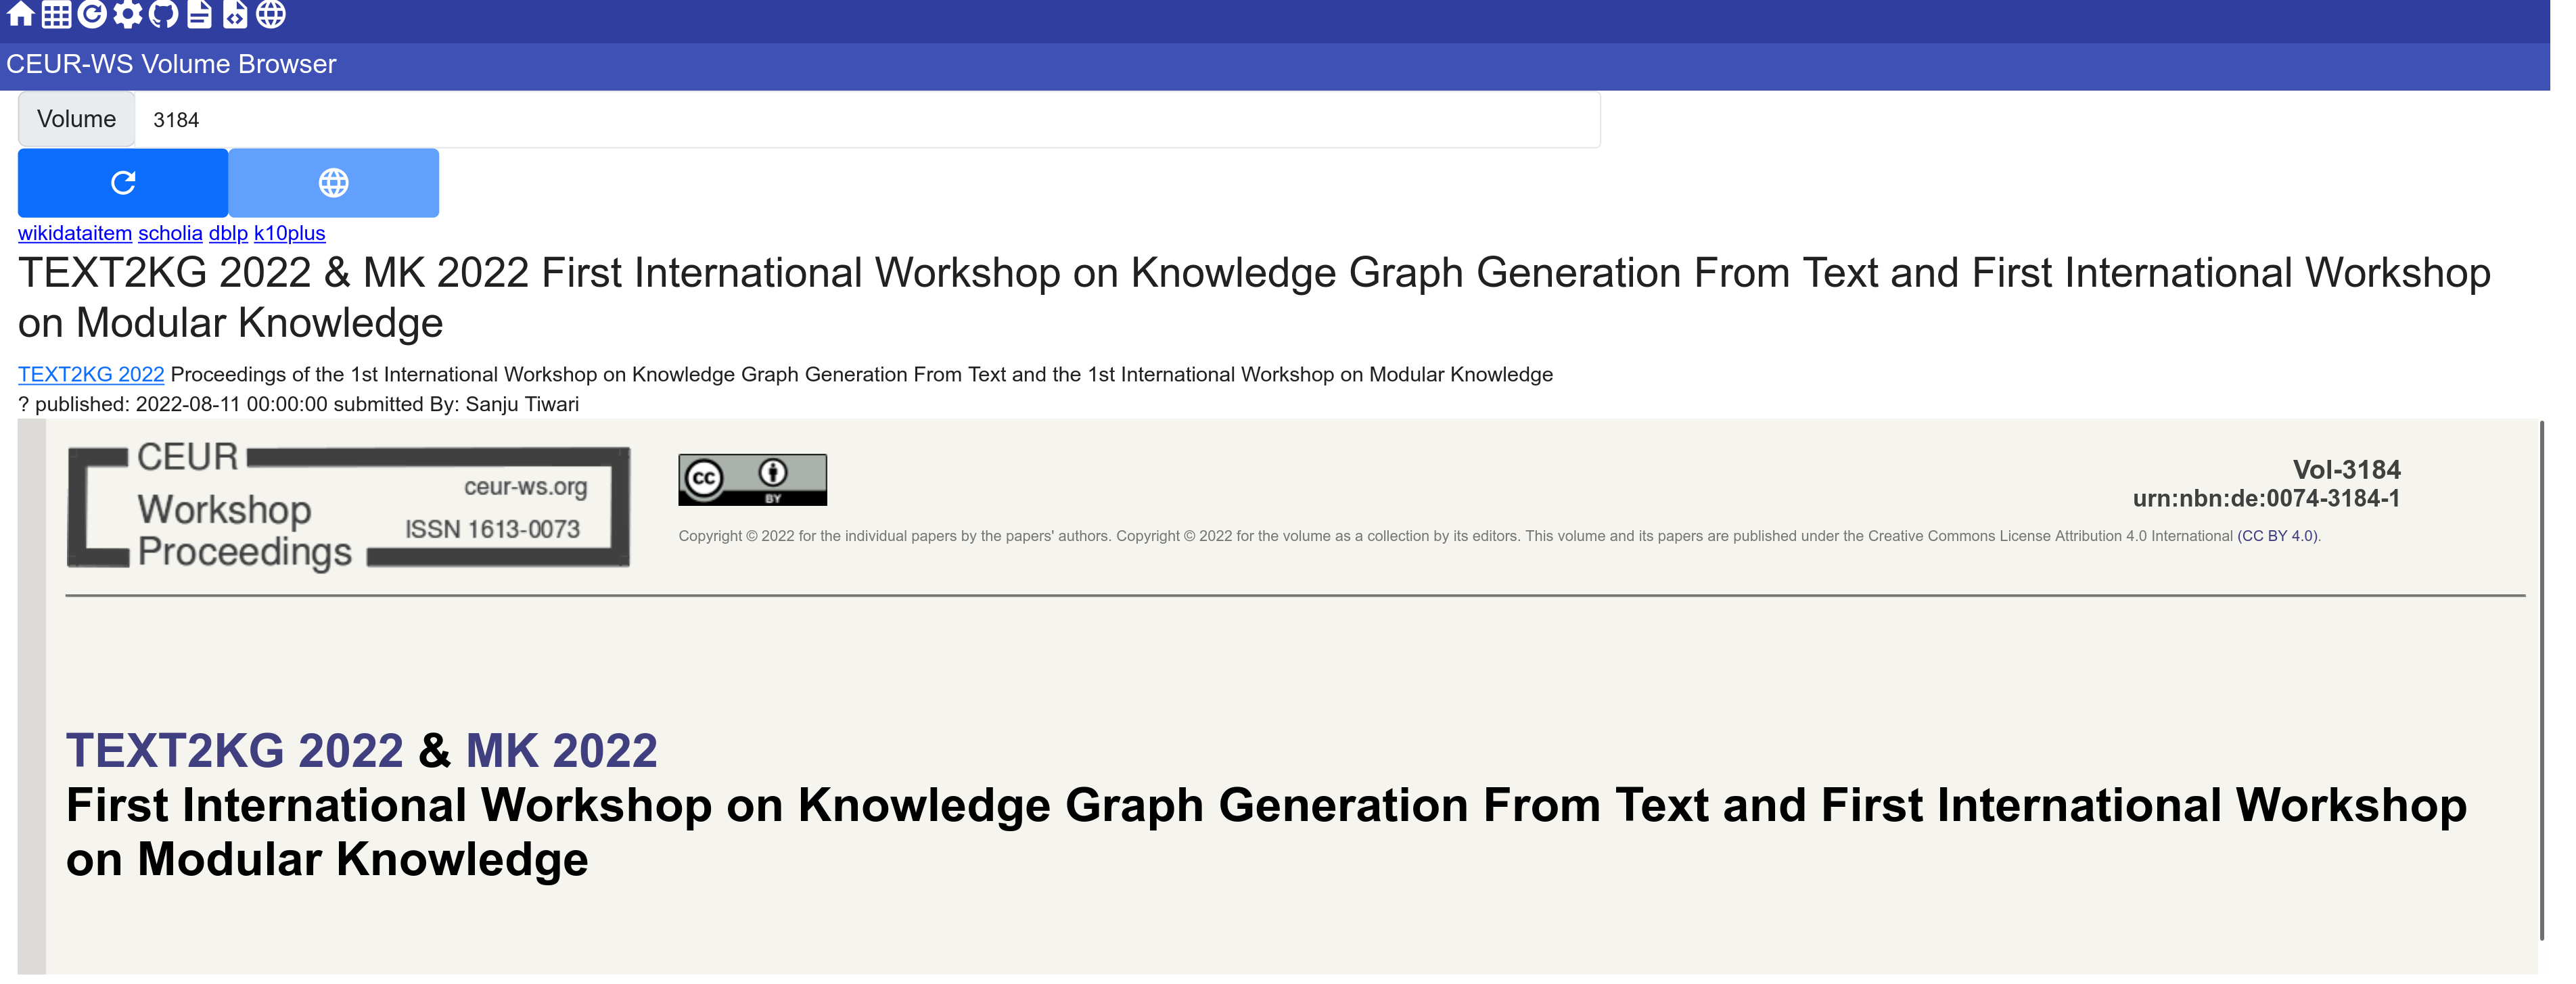
\includegraphics[width=\linewidth]{cvb_screenshot.png}
    \caption{Screenshot of CEUR-WS Volume Browser}
    \label{fig:cvb_screenshot}
\end{figure}
Figure~\ref{fig:cvb_screenshot} shows a screen shot of the CEUR-WS Volume Browser which we created as a means to support semantification tasks such as transferring meta-data of recently added volumes to Wikidata as well as showing the available index entries for volumes that have been published for a few weeks/months already. The example shown is for \footnotelink{https://ceur-ws.org/Vol-3262/}{CEUR-WS Volume 3262 Wikidata Workshop 2022}.  

\begin{figure}[ht]
    \centering
    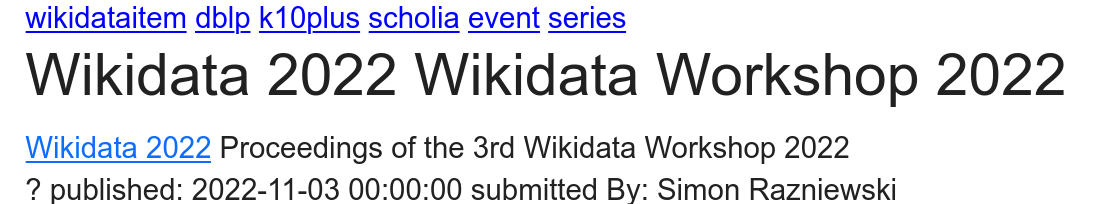
\includegraphics[width=0.7\linewidth]{cvb_volume_browser_enlarged.png}
    \caption{CEUR-WS Volume Browser enlarged details with links to external KGs}
    \label{fig:cvb_details}
\end{figure}
Figure~\ref{fig:cvb_details} shows an enlarged section of the screenshot where the links between the proceedings volumes and the external knowledegraphs are presented. For the example these are \footnotelink{http://www.wikidata.org/entity/Q115053286}{wikidataitem}, \footnotelink{https://dblp.org/db/conf/semweb/wikidata2022}{dblp}, \footnotelink{https://opac.k10plus.de/DB=2.299/PPNSET?PPN=1830580760}{k10plus}, and the scholia links to the proceedings, event and \footnotelink{https://scholia.toolforge.org/event-series/Q106429025}{event series} (which has links to the event and proceedings). 
\subsection{CEUR-WS Semantic MediaWiki}
\begin{figure}[ht]
    \centering
    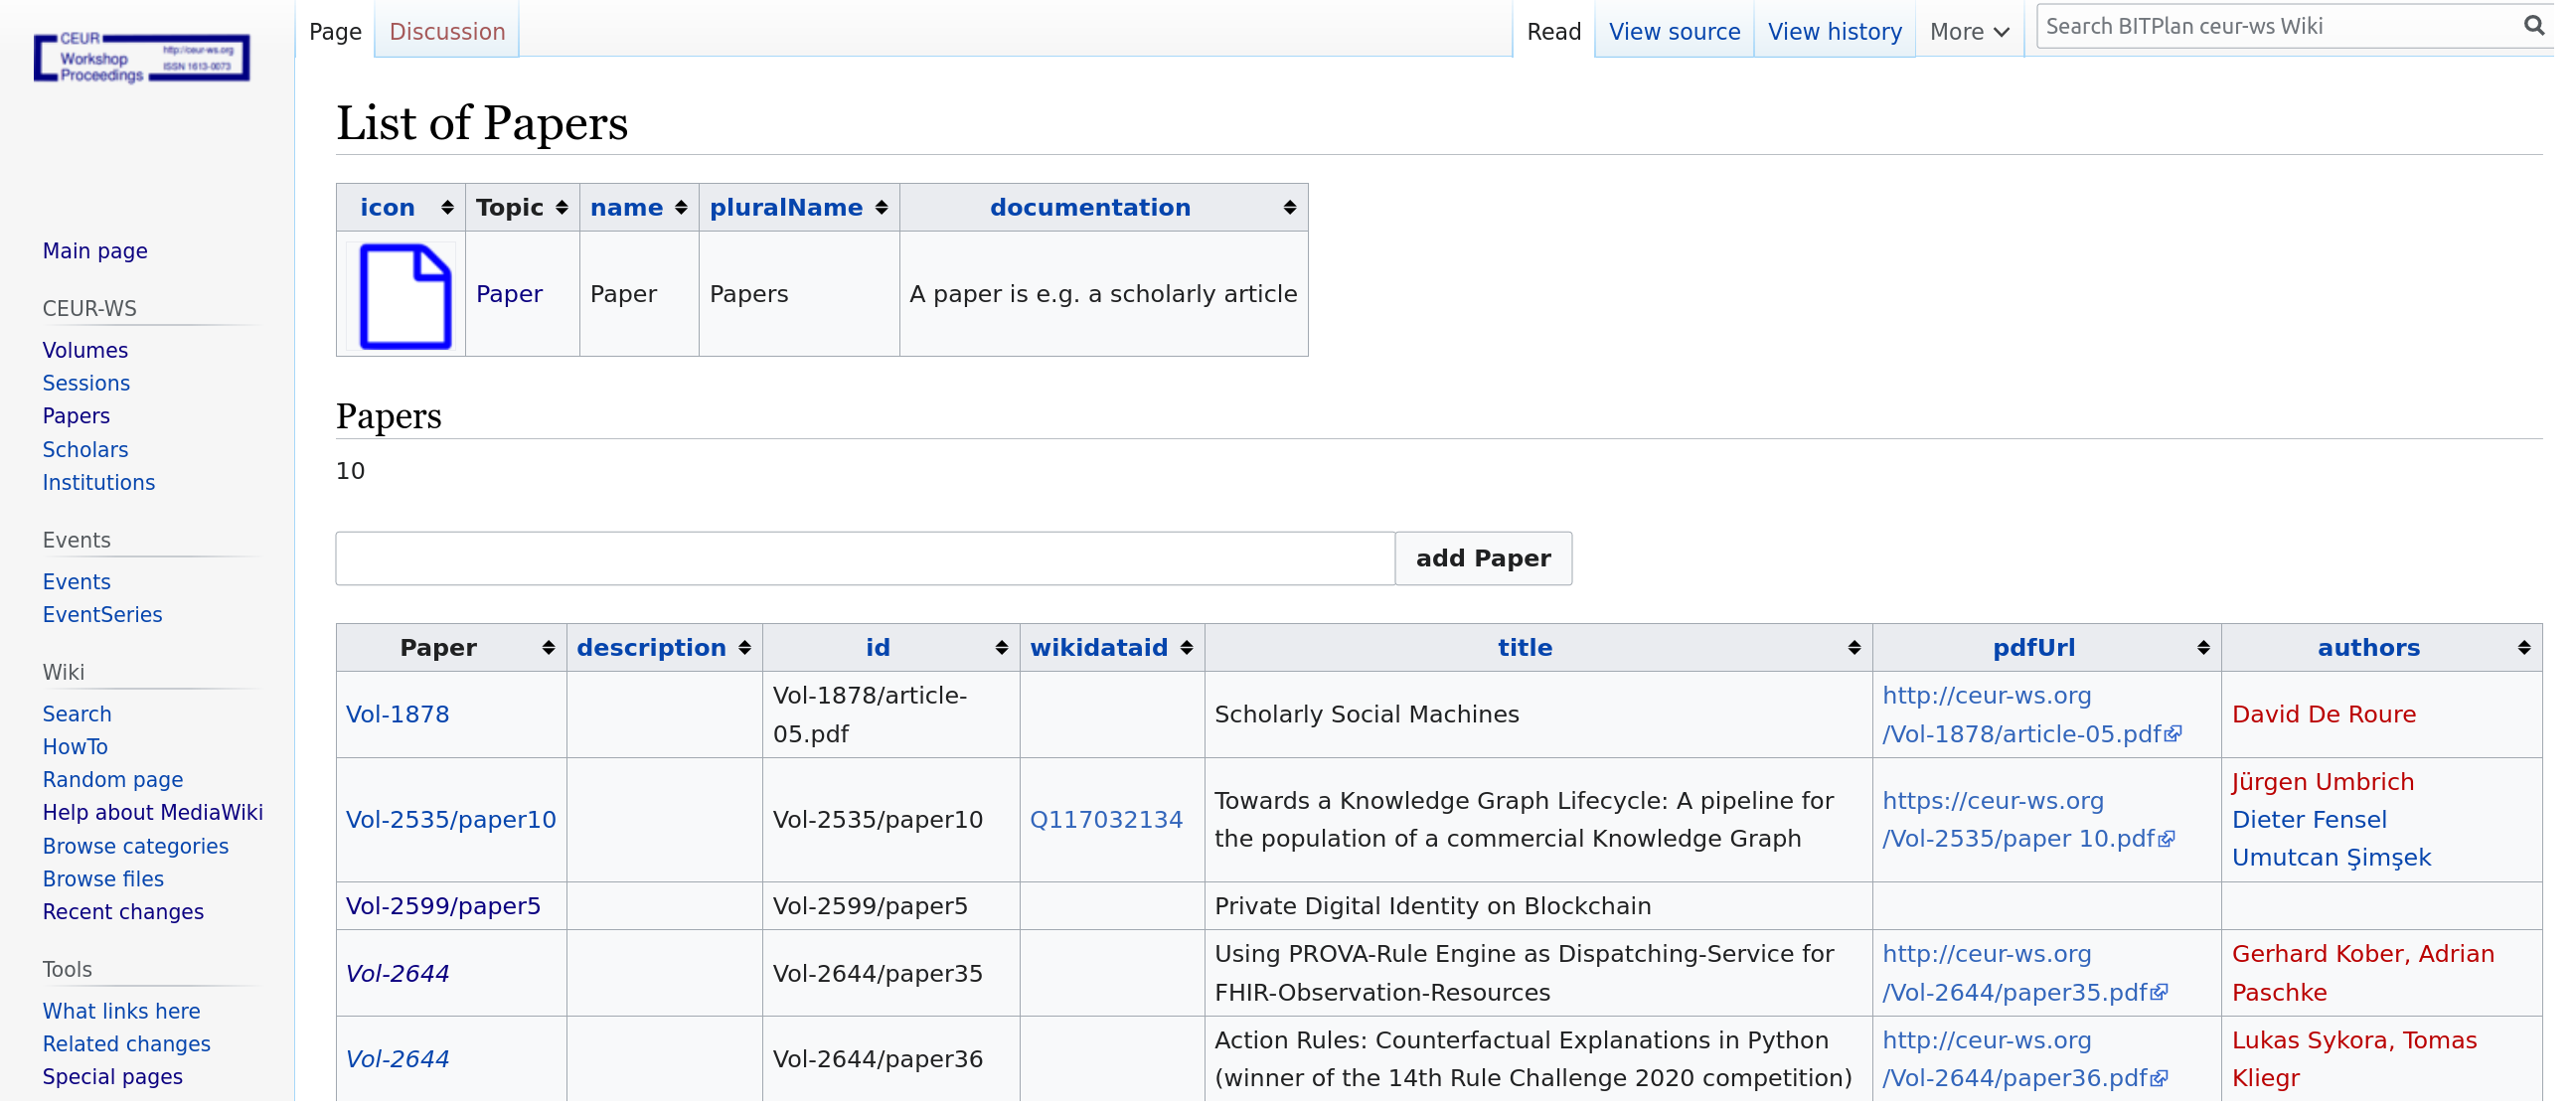
\includegraphics[width=\linewidth]{ceurws_wiki_list_of_papers.png}
    \caption{List of Papers in the CEUR-WS Semantic MediaWiki}
    \label{fig:ceurws_wiki}
\end{figure}
The CEUR-WS Semantic MediaWiki is available as a prototype as depicted in Figure~\ref{fig:ceurws_wiki} that shows how a content management system approach may be applied to the metadata, which allows for new features such as full text search. Semantic MediaWiki is a useful prototyping tool, since it allows to try out semantic properties and relations that are not yet fit for full public exposure via Wikidata. 
The example screenshot shows how a MediaWiki displays links with non-existing targets in red, allowing to judge the coverage of the disambiguation easily. 

\section{Results}\label{sec:Results}

\subsection{Disambiguation}
With our extraction method for editors we are able to obtain 11,764 editor signatures from 3354 volumes.
Comparing these signatures against the editor records, we were able to query from dblp, it showed that 9321 signatures (4942 unique editors) can be linked to dblp and thus have at least a \wdp{DBLP author id}{P2456}.
For 2233 volumes this means that all their editors can be extracted and disambiguated to a dblp author id.
But it also showed that for 387 volumes the extraction method returned fewer editors as defined in dblp with the majority of these volumes being the early 500 volumes which were manually created with a high variety in format.

With the goal to enter the editors into Wikidata, the editor signature also needs to be disambiguated to a Qid.
Having the DBLP author id greatly helps in the disambiguation process as it allows to query dblp for more person identifier.
This list of identifiers can than be used to query Wikidata to check if a person exists with at least on of those identifiers.
The check against Wikidata showed that 1467 editors could be identified and it also showed 62 conflicting items.
We found that dblp's coverage of person metadata synchronized with Wikidata is already leading to only 77  CEUR-WS editors missing.
%The conflict can either mean that dblp describes more than one person with one id or Wikidata.
%Comparing the editors we found in Wikidata based on all the ids dblp provides we only found 77 additional editors suggesting that dblp already synchronizes the person identifiers with Wikidata if a link is established.
Applying the disambiguation results and linking to CEUR-WS and dblp metadata will require mass editing of Wikidata via a special CEUR-WS bot, which requires approval by Wikidata before being applicable in the next project phase. 

\subsection{Metadata Query capability}
Having the CEUR-WS metadata available in Wikidata allows for standard SPARQL queries, e.g., using the Wikidata Query Service to be applied to analyze it. Figure~\ref{fig:cvb_screenshot} shows a map of the distribution of event locations created with such a query. 
\begin{figure}
    \centering
    %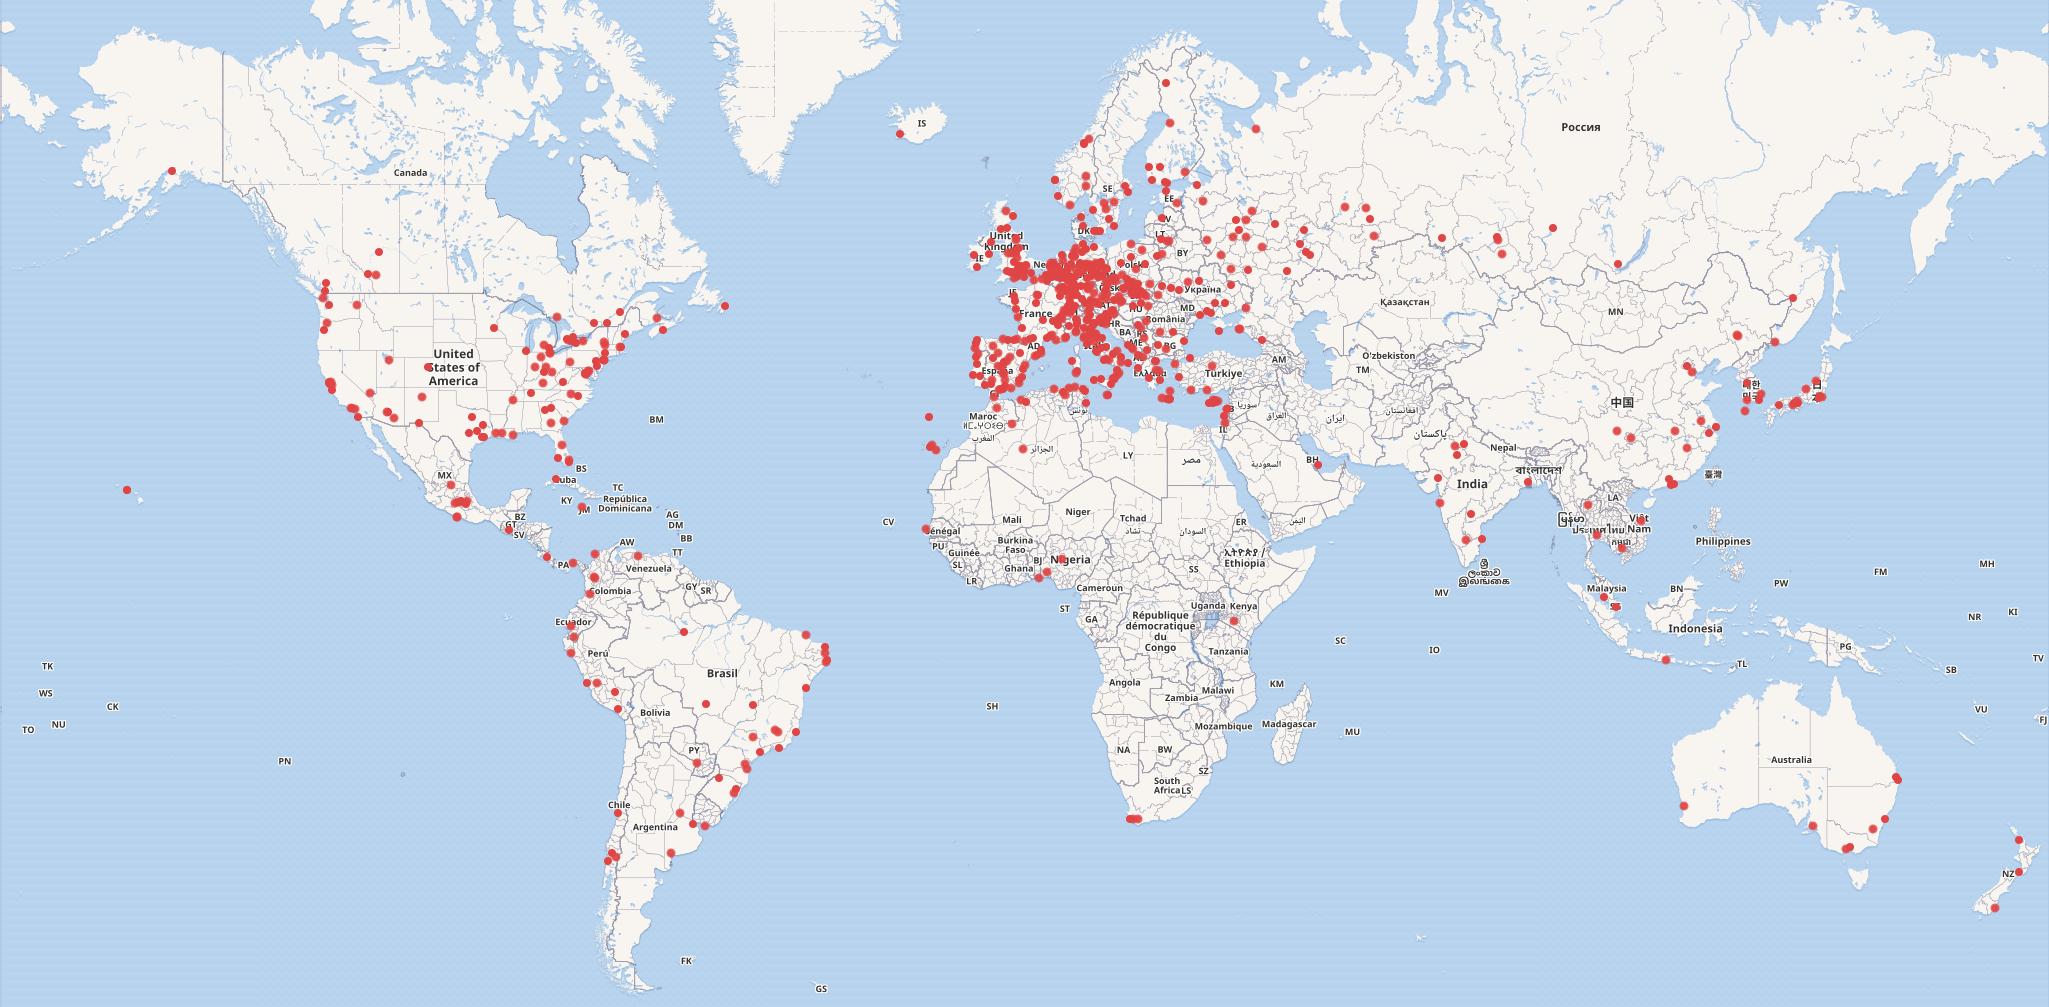
\includegraphics[width=\linewidth]{ceur-ws_events_map.png}
    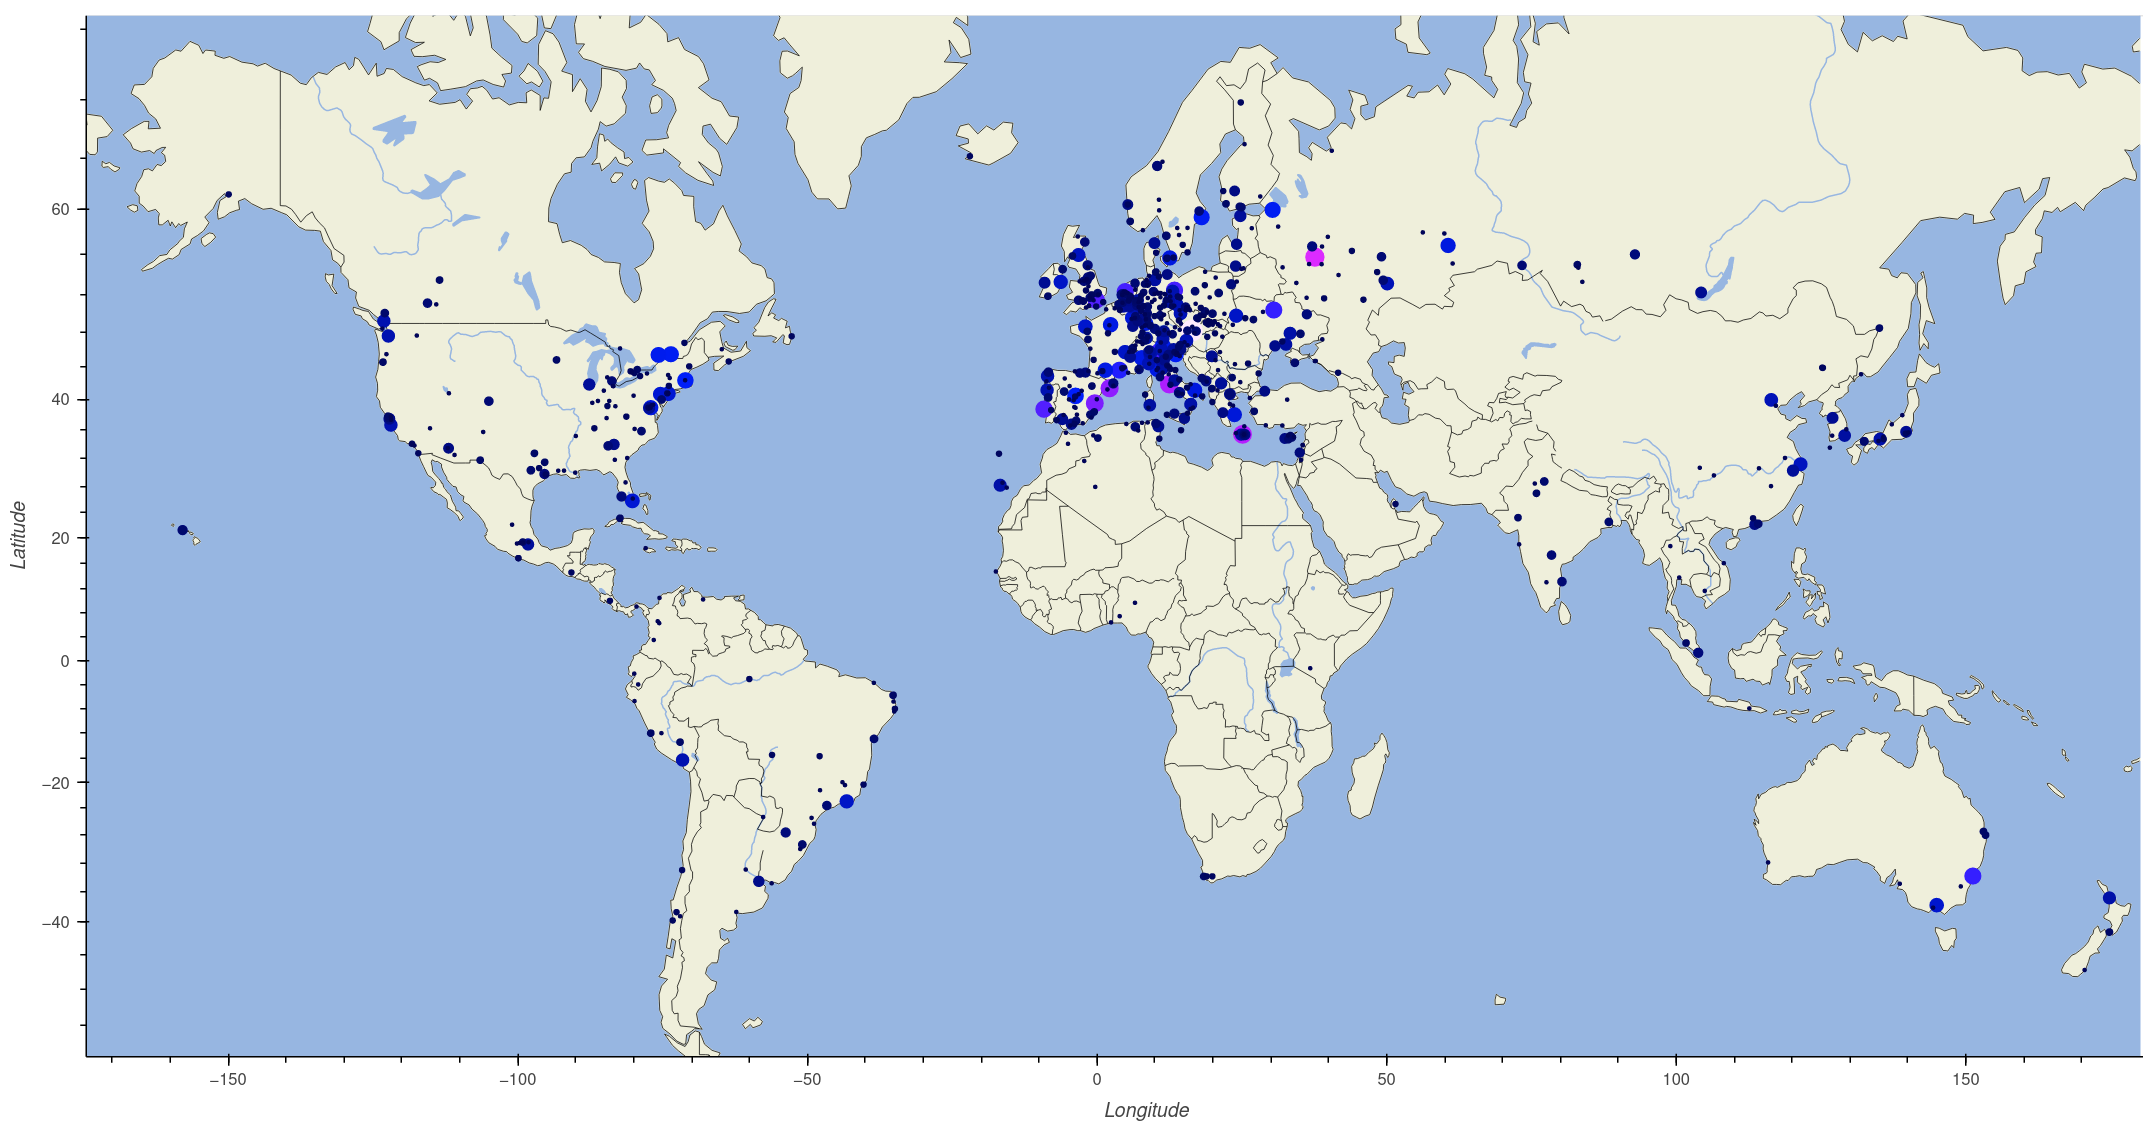
\includegraphics[width=0.8\linewidth]{ceurws_event_locations_alternative.png}
    \caption{Locations of all CEUR-WS proceedings events (\href{https://w.wiki/678Q}{WDQS Query})}
    \label{fig:event_map}
\end{figure}
The relevance of the original set of 20 queries for Task~1 that were set as a benchmark in 2014 for different stakeholders was subjectively rated by us to \footnotelink{https://cr.bitplan.com/index.php/List\_of\_Queries}{sort the queries by priority}. The most relevant queries and the 5 queries Q1.5, Q1.12, Q1.13, Q1.16 and Q1.17 that rely on the main index have been implemented as \footnotelink{https://cr.bitplan.com/index.php/Semantic\_Publishing\_Challenge\_Queries}{SPARQL queries} that are compatible with the Wikidata Query Service endpoint to prove that our approach covers the intentions of the original challenge.  Our result supplies even more capabilities given the option to do federated SPARQL queries over the connected Wikidata, dblp and k10plus knowledge graphs. The use of Wikidata ids as persistent identifiers is a core success factor here.

\subsection{Further Evaluation}
Making the CEUR-WS Volume metadata available on Wikidata has improved the indexing Coverage to 100\% of all valid Volumes compared to 69\% for k10plus and  76\% for dblp.

%Check against dblp/k10plus (wikicfp) ...

The timeliness of the CEUR-WS metadata in Wikidata is much higher than for dblp or k10plus. For dblp it takes a few days to weeks, for k10plus it may take weeks to months before the metadata shows up. The Wikidata update may be done immediately when publishing with no delay. With the separation of event and proceeding entries it is now possible to show future events for which there are no proceedings available yet as soon as the events have been announced and later link the detailed proceedings metadata to the event record.

\section{Conclusion}\label{sec:Conclusion}
We have presented the first steps of CEUR-WS Semantification that result in the metadata of CEUR-WS Volumes being available in Wikidata. The linking of the relevant entities for workshops, the conferences these workshops might be colocated with, the event series the workshops and events might form as well as the linking to editor, author and paper entries and the affiliated institutions has been prototyped. 

The cross-linking with dblp and k10plus has been performed and may now be continuously applied in the future.

Given that all four involved meta data sources -- CEUR-WS, Wikidata, dblp and k10plus -- have a lot of manual curation involved, data quality errors which derive from human errors still have to be mitigated with the goal to achieve a lower error rate than would be possible with manual efforts alone.

\subsection{Future Work}
\begin{figure}
    \centering
    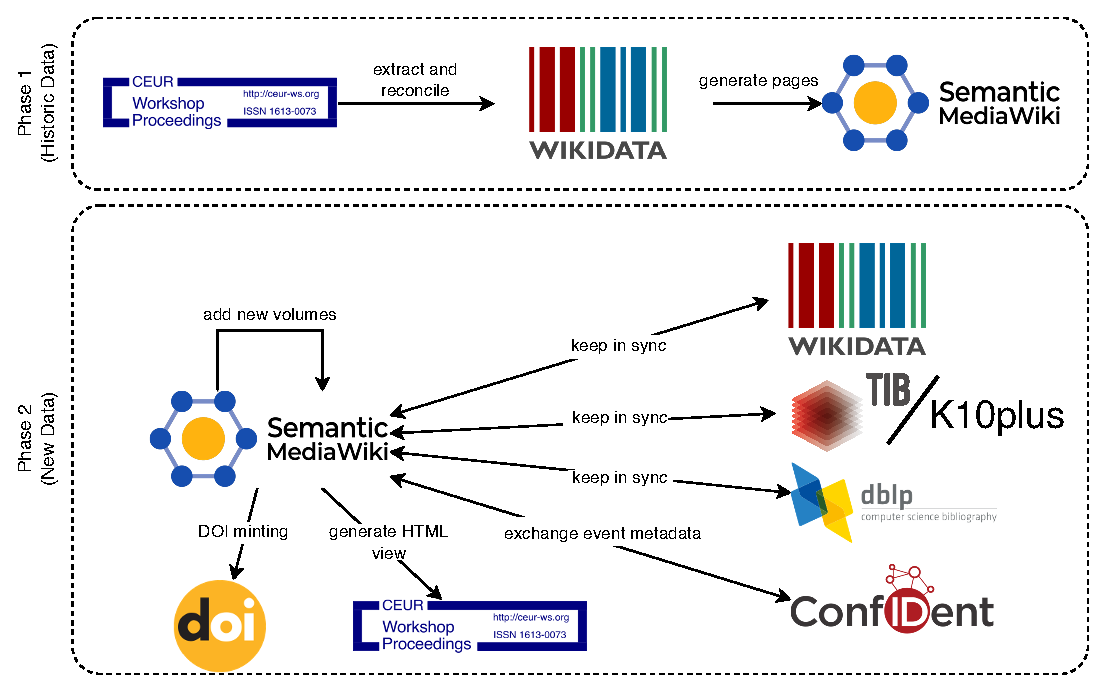
\includegraphics[width=0.8\linewidth]{CEUR-WS-SemantificationOverview.eps}
    \caption{CEUR-WS Semantification}
     \label{fig:sem_overview}
\end{figure}

Figure~\ref{fig:sem_overview} shows an overview of a possible new approach to publishing via CEUR-WS. The core idea is to separate the concerns for displaying the content (static HTML/Semantic MediaWiki) from the storage of the metadata in a knowledge graph, e.g., Wikidata. 

The new publishing workflow shall be based on single-point-of-truth metadata that is kept in computer readable format such as JSON and generate the HTML presentation from this metadata. 

CEUR-WS papers do not have DOIs assigned to them during the publishing process. Assigning DOIs to papers is a feature much asked for by workshop organizers these days which CEUR-WS did not supply in the past. The new approach/architecture would simplify the DOI minting since the necessary metadata is a subset of the metadata we intend to provide anyway.

The first phase shows the current state of the workflow in the prototype phase which we report on in this paper, while the second phase is the goal of the \tquote{Semantification} project hat has been officially started in February 2023 by the CEUR-WS Editors team. 

\ifreview
\else
\paragraph{Acknowledgements.}
Main open source libraries being used by the work described:
\footnotelink{https://pypi.org/project/beautifulsoup4/}{BeautifulSoup4}, \footnotelink{https://github.com/LibreCat/Catmandu}{Catemandu}, \footnotelink{https://github.com/justpy-org/justpy}{justpy}, \footnotelink{https://github.com/somnathrakshit/geograpy3}{geograpy3}
\hiddenfootnotelink{https://github.com/WolfgangFahl/py-yprinciple-gen}{https://tinyurl.com/26ufkm49}{py-yprinciple-gen}

We would like to thank Jakob Voß for helping with the k10plus matching and creating the Wikidata property \wdp{colocated with}{P11633} in due time.

This paper is dedicated to the memory of CEUR-WS board member Ralf Klamma $\dag$ January 2023.

This research has been partly funded by a grant of the Deutsche Forschungsgemeinschaft (DFG). \footnote{\href{https://gepris.dfg.de/gepris/projekt/426477583}{ConfIDent project; see https://gepris.dfg.de/gepris/projekt/426477583}}
\fi
% Bibliography
\bibliography{text2kg2023.bib}

\end{document}
